\documentclass[11pt]{article}
\usepackage[scaled=0.92]{helvet}
\usepackage{geometry}
\geometry{letterpaper,tmargin=1in,bmargin=1in,lmargin=1in,rmargin=1in}
\usepackage[parfill]{parskip} % Activate to begin paragraphs with an empty line rather than an indent %\usepackage{graphicx}
\usepackage{amsmath,amssymb, mathrsfs,  mathtools, dsfont}
\usepackage{tabularx}
\usepackage{tikz-cd}
\usepackage[font=footnotesize,labelfont=bf]{caption}
\usepackage{graphicx}
\usepackage{xcolor}
%\usepackage[linkbordercolor ={1 1 1} ]{hyperref}
%\usepackage[sf]{titlesec}
\usepackage{natbib}
\usepackage{../../Tianpei_Report}

%\usepackage{appendix}
%\usepackage{algorithm}
%\usepackage{algorithmic}

%\renewcommand{\algorithmicrequire}{\textbf{Input:}}
%\renewcommand{\algorithmicensure}{\textbf{Output:}}



\begin{document}
\title{Lecture 4: Empirical Processes}
\author{ Tianpei Xie}
\date{Feb. 1st., 2023}
\maketitle
\tableofcontents
\newpage
\section{Uniform Law of Large Numbers}
\subsection{Motivations}
\begin{itemize}
\item \begin{remark}(\textbf{\emph{Unbiased Estimator of Cumulative Distribution Function}})\\
The law of any scalar random variable $X$ can be fully specified by its \emph{\textbf{cumulative distribution function (CDF)}}, whose value at any point $t \in \bR$ is given by $F(t) := \cP[X \le t]$. Now suppose that we are given a collection $\set{X_i}^{n}_{i=1}$ of $n$ i.i.d. samples, each drawn according to the law specified by $F$. A natural \emph{estimate} of $F$ is \emph{\textbf{the empirical CDF}} given by
\begin{align}
\widehat{F}_n(t) &:=\frac{1}{n}\sum^{n}_{i=1}\mathds{1}_{(-\infty, t]}(X_i),\label{def: empirical_cdf}
\end{align} where $\mathds{1}_{(-\infty, t]}(x)$ is a $\set{0, 1}$-valued indicator function for the event $\set{x \le t}$. Since \emph{\textbf{the population CDF}} can be written as $F(t) = \E{}{\mathds{1}_{(-\infty, t]}(X)}$, the empirical CDF is an \emph{\textbf{unbiased estimate}}.

For each $t \in \bR$, \emph{\textbf{the strong law of large numbers}} suggests that 
\begin{align*}
\widehat{F}_n(t) \rightarrow F(t), \quad \text{ a.s.}
\end{align*} A natural goal is to strengthen\emph{ this pointwise convergence} to a form of \emph{\textbf{uniform convergence}}. The reason why uniform convergence of $\widehat{F}_n(t)$ to $F(t)$ is important is that it can be used to prove the \emph{\textbf{consistency}} of \emph{\textbf{plug-in estimator}} for \emph{functionals of distribution function}.
\end{remark}

\item \begin{example} (\textbf{\emph{Expectation Functionals}}) \\
Given some integrable function $g$, we may define \underline{\textbf{\emph{the expectation functional}}} $\gamma_g$ via
\begin{align}
\gamma_{g}(F) &:= \int g(x) dF(x). \label{def: exp_functional}
\end{align} For any g, \emph{the plug-in estimate} is given by $\gamma_g(\widehat{F}_n) = \frac{1}{n}\sum^{n}_{i=1}g(X_i)$, corresponding to \emph{\textbf{the sample mean}} of $g(X)$. 
\end{example}

\item \begin{example} (\textbf{\emph{Quantile Functionals}}) \\
For any $\alpha \in [0, 1]$, \underline{\textbf{\emph{the quantile functional}}} $Q_{\alpha}$ is given by
\begin{align}
Q_{\alpha}(F) &:= \inf\set{t \in \bR: F(t) \ge \alpha}. \label{def: quantile_functional}
\end{align} The \emph{\textbf{median}} corresponds to the special case  $\alpha= 0.5$. \emph{The plug-in estimate} is given by
\begin{align}
Q_{\alpha}(\widehat{F}_n) &:= \inf\set{t \in \bR: \frac{1}{n}\sum^{n}_{i=1}\mathds{1}_{(-\infty, t]}(X_i) \ge \alpha}  \label{def: quantile_functional_estimate}
\end{align} and corresponds to estimating the $\alpha$-th quantile of the distribution by \emph{the $\alpha$-th \textbf{sample quantile}}. In the special case $\alpha= 0.5$, this estimate corresponds to \emph{the sample median}.  In this case, $Q_{\alpha}(\widehat{F}_n)$ is a fairly complicated, \emph{nonlinear function of all the
variables}, so that this convergence does not follow immediately by a classical result such as the law of large numbers.
\end{example}

\item \begin{example}(\emph{\textbf{Goodness-of-fit Functionals}})\\
It is frequently of interest to test the hypothesis of whether or not a given set of data has been drawn from a known distribution $F_0$. Such tests can
be performed using \emph{functionals that \textbf{measure the distance} between $F$ and the target CDF $F_0$}, including \emph{the sup-norm distance} $\norm{F - F_0}{\infty}$, or other distances such as \emph{\textbf{the Cramer-von Mises criterion}} based on the functional 
\begin{align*}
\gamma_{g}(F) &:= \int_{-\infty}^{+\infty} \paren{F(x) - F_0(x)}^2 dF_0(x)
\end{align*}
\end{example}

\item \begin{remark} (\emph{\textbf{Consistency of Plug-In Estimate}})\\
For any \emph{\textbf{plug-in estimator}} $\gamma_g(\widehat{F}_n)$, an important question is to understand when it is \emph{\textbf{consistent}} -- that is, when does $\gamma_g(\widehat{F}_n)$ converge to $\gamma_{g}(F)$ in \emph{probability} (or \emph{almost surely})?

We can define \emph{the \textbf{continuity} of a \textbf{functional}} $\gamma$ with respect to \emph{the supremum norm}: more precisely, we say that the functional $\gamma$ is \emph{\textbf{continuous} at $F$ in the \textbf{sup-norm}} if, for all $\epsilon > 0$, there exists a $\delta > 0$ such that 
\begin{align*}
\norm{G - F}{\infty} := \sup_{t\in \bR}\abs{G(t) - F(t)} \le \delta  \quad \text{ implies that }\quad \abs{\gamma(G) - \gamma(F)} \le \epsilon.
\end{align*} 
Thus for any \emph{\textbf{continuous functional}}, it reduces the \emph{\textbf{consistency}} question for \emph{the plug-in estimator} $\gamma_g(\widehat{F}_n)$ to the issue of whether or not the random variable $\|\widehat{F}_n - F\|_{\infty}$ \emph{\textbf{converges to zero}}. 
\end{remark}
\end{itemize}
\subsection{Glivenko-Cantelli Theorem}
\begin{itemize}
\item \begin{theorem} (\textbf{Glivenko-Cantelli Theorem})  \citep{wellner2013weak, wainwright2019high, gine2021mathematical} \\ 
For any distribution, the empirical CDF 
\begin{align*}
\widehat{F}_n(t) &:=\frac{1}{n}\sum^{n}_{i=1}\mathds{1}_{(-\infty, t]}(X_i)
\end{align*}  is a \textbf{strongly consistent estimator} of the population CDF in \textbf{the uniform norm}, meaning that
\begin{align}
\norm{\widehat{F}_n - F}{\infty} := \sup_{t\in \bR}\abs{\widehat{F}_n(t) - F(t)} \rightarrow 0, \text{ a.s. } \label{eqn: gilvenko_cantelli}
\end{align}
\end{theorem}

\item \begin{remark}(\textbf{\emph{Uniform Law of Large Numbers}})\\
\emph{\textbf{The Glivenko-Cantelli theorem}} \emph{generalizes} \emph{\textbf{the strong law of large numbers}} to \emph{stochastic process}. It confirms that the \emph{convergence} of sample mean $\cP_n f$ to its expectation $\cP f$ is true in function space $\cF$ not only \emph{in \textbf{pointwise topology}} but also \emph{in \textbf{uniform topology}}. Thus,  \emph{the Glivenko-Cantelli theorem} is also called \emph{\textbf{the uniform law of large numbers}}.
\end{remark}
\end{itemize}


\section{Empirical Processes}
\subsection{Definitions}
\begin{itemize}
\item \begin{definition}(\textbf{\emph{Empirical Measure}})  \citep{wellner2013weak, gine2021mathematical} \\
Let $(\cX, \srF, \cP)$ be a \emph{probability space}, and let $X_i, i \in \bN$, be the \emph{coordinate functions} of \emph{the \textbf{infinite product probability space}} $(\Omega, \srB,  \bP) := (\cX^{\infty}, \srF^{\infty}, \cP^{\infty})$,  $X_i :  \cX^{\infty} \to \cX$, which are \emph{\textbf{independent} identically distributed} $\cX$-valued random variables with law $\cP$. %In fact, we will always take \emph{independent variables} (equally distributed or not) to be \emph{the coordinate functions} on \emph{product probability spaces}.

\underline{\emph{\textbf{The empirical measure}}} corresponding to the `\emph{observations}' $X_1 \xdotx{,} X_n$, for any $n \in \bN$, is defined as \emph{\textbf{the \underline{random} discrete probability measure}}
\begin{align}
\cP_n &:= \frac{1}{n}\sum_{i=1}^{n}\delta_{X_i} \label{def: empirical_measure}
\end{align} where $\delta_x$ is \emph{Dirac measure} at $x$, that is, unit mass at the point $x$.  In other words, for each event $A$,  $\cP_n(A)$ is \emph{the \textbf{proportion} of \textbf{observations} $X_i$,  $i = 1 \xdotx{,} n$, that fall in $A$}; that is,
\begin{align*}
\cP(A) &= \frac{1}{n}\sum_{i=1}^{n}\delta_{X_i}(A) = \frac{1}{n}\sum_{i=1}^{n}\ind{X_i \in A}, \quad A \in \srF.
\end{align*}
\end{definition}

\item \begin{remark}(\textbf{\emph{Probability Measure with Operator Notation}}) \citep{wellner2013weak, gine2021mathematical} \\
For any measure $\mu$ and $\mu$-integrable function $f$, we will use the following \underline{\textbf{\emph{operator notation}}} for the integral of $f$ with respect to $\mu$:
\begin{align*}
\mu f \equiv \mu(f) =  \int_{\Omega} f d\mu.
\end{align*} This is valid since there exists an isomorphism between \emph{the space of probability measure} and \emph{the space of bounded linear functional} on $\cC_{0}(\Omega)$ by Riesz-Markov representation theorem (assuming $\Omega$ is \emph{locally compact}). By this notion the expectation $ \cP f = \E{\cP}{f}$.
\end{remark}

\item \begin{definition} (\textbf{\emph{Empirical Process}})  \citep{wellner2013weak, gine2021mathematical} \\
Let $\cF$ be a \emph{collection of $\cP$-integrable functions} $f: \cX \to \bR$, usually infinite. For any such class of functions $\cF$, \underline{\emph{\textbf{the empirical measure}}} defines a \emph{\textbf{stochastic process}}
\begin{align}
f \rightarrow \cP_{n}f, \quad f\in \cF \label{def: empirical_process}
\end{align} which we may call  \underline{\emph{\textbf{the empirical process indexed by $\cF$}}}, although we prefer to reserve the
notation `\emph{empirical process}' for \emph{the \textbf{centred} and \textbf{normalised} process}
\begin{align}
f \rightarrow \nu_{n}(f) :=\sqrt{n} \paren{\cP_n f - \cP f}, \quad f\in \cF. \label{def: centered_empirical_process}
\end{align}
\end{definition}

\item \begin{remark}
An explicit notion of \emph{(centered and normalized) empirical process} is
\begin{align*}
\sqrt{n} \paren{\cP_n f - \cP f} \equiv \frac{1}{\sqrt{n}}\sum_{i=1}^n\paren{f(X_i) - \E{\cP}{f(X)}}, \quad f\in \cF.
\end{align*} where $X_1 \xdotx{,} X_n \sim \cP$ are i.i.d random variables. Note that it is a stochastic process since \emph{the function $f$ is changing} in $\cF$, i.e. the process $\paren{\cP_n  - \cP}f$ is indexed by function $f \in \cF$ not finite dimensional variable.
\end{remark}



\item \begin{remark}(\textbf{\emph{Random Measure on Function Space $\cF$}})\\
Normally we assume that data are sampled from some distribution $\cP$ and the data itself is random. However, the empirical measure 
\begin{align*}
\cP_n &:= \frac{1}{n}\sum_{i=1}^{n}\delta_{X_i}
\end{align*} itself is considered as a \emph{\textbf{random}} probability measure. That is, \emph{the sampling mechanism itself contains randomness} and it is not sampling from one distribution but \emph{\textbf{a system of distributions depending on the choice of dataset $X_1 \xdotx{,} X_n$ }}, which in turn were sampled from some \emph{prior} $\cP$. Due to this randomness, $\cP_n f = \E{\cP_n}{f}$ is not a fixed expectation number but a random variable. For given $f\in \cF$, this is the empirical mean (i.e. sample mean)
\begin{align*}
\cP_n f = \E{\cP_n}{f} = \frac{1}{n}\sum_{i=1}^n f(X_i).
\end{align*} \emph{\textbf{The critical difference}} between \emph{empirical process} vs. \emph{sample mean} is that the \emph{\textbf{latter}} assume that  $f$ is \emph{\textbf{fixed}}, while the former is defined with respect to \emph{\textbf{a class of functions}} $\cF$.
\end{remark}

\item \begin{remark}
Note that we can always associated a stochastic process $(X_t)_{t\in T}$ with a function class $\cF$ indexed by $T$ as
\begin{align*}
X_t = f_t(Z), \quad f_t \in \cF, t \in T \quad &\Rightarrow  \quad \sum_{i=1}^n X_{i,t} = \sum_{i=1}^n f_t(Z_i) = \cP_n f_t,  \quad t\in T
\end{align*} where $Z_i$ is the \emph{\textbf{state}} of  stochastic process $(X_{i,t})_{t\in T}$. Thus an empirical process $\cP_n f_t$ can be seen as the \emph{\textbf{sum}} of $n$ \emph{\textbf{independent stochastic processes}} $\set{(X_{i,t})_{t\in T}}_{i =1}^{n}$. 

An \emph{\textbf{empirical process}} is a \underline{\emph{\textbf{stochastic process}}} that \emph{describes \underline{the \textbf{proportion} of objects} in a system \underline{\textbf{in a given state}}}.  Applications of the theory of empirical processes arise in \emph{\textbf{non-parametric statistics}}.
\end{remark}

\item \begin{remark} (\emph{\textbf{Object of Empirical Process Theory}}) \\
\emph{The \textbf{object} of empirical process theory} is to study \emph{the \textbf{properties} of the \textbf{approximation}} of $\cP f$ by $\cP_n f$, \emph{\textbf{uniformly in $\cF$}}, concretely, to obtain both \emph{\textbf{probability estimates} for the random quantities}
\begin{align*}
\norm{\cP_n  - \cP}{\cF} &:= \sup_{f \in \cF}\abs{\cP_n f - \cP f}
\end{align*}
and \emph{\textbf{probabilistic limit theorems}} for the processes $\set{ (\cP_n - \cP)(f) : f \in \cF}$.

Note that the quantity $\norm{\cP_n  - \cP}{\cF}$ is a \emph{\textbf{random variable}} since $\cP_n$ is a \emph{\textbf{random measure}}.
\end{remark}

\item \begin{remark} (\textbf{\emph{Measurability Problem}})\\
There may be a \emph{\textbf{measurability problem}} for 
\begin{align*}
\norm{\cP_n  - \cP}{\cF} &:= \sup_{f \in \cF}\abs{\cP_n f - \cP f}
\end{align*}  since \emph{the \textbf{uncountable} suprema} of measurable functions \emph{may not be measurable}. 

However, there are many situations where this is actually a \emph{\textbf{countable supremum}}. For instance, for probability distribution on $\bR$
\begin{align*}
\norm{\cP_n  - \cP}{\infty} &:= \sup_{t \in \bR}\abs{\paren{\cP_n - \cP}(-\infty, t)} =  \sup_{t \in \bQ}\abs{F_n(t) - F(t)} =  \sup_{t \in \bQ}\abs{\paren{\cP_n - \cP}(-\infty, t)}
\end{align*} where $F(t) = \cP\paren{-\infty, t}$ is the cumulative distribution function. If $\cF$ is \emph{countable} or if there exists $\cF_0$ \emph{countable} such that
\begin{align*}
\norm{\cP_n  - \cP}{\cF}  = \norm{\cP_n  - \cP}{\cF_0}, \quad \text{a.s.} 
\end{align*} then the measurability problem disappears. For the next few sections we will simply \emph{\textbf{assume}} that the class $\cF$ is \emph{\textbf{countable}}.
\end{remark}

\item \begin{remark} (\textbf{\emph{Bounded Assumption}})\\
If we assume that
\begin{align}
\sup_{f \in \cF}\abs{f(x) - \cP f} < \infty, \quad \forall x \in \cX, \label{def: empirical_process_bounded}
\end{align}
then the maps from $\cF$ to $\bR$,
\begin{align*}
f \rightarrow f(x) - \cP f, \quad x\in \cX,
\end{align*} are \emph{\textbf{bounded functionals}} over $\cF$, and therefore, so is $f \to  (\cP_n - \cP)(f)$. That is,
\begin{align*}
\cP_n - \cP \in \ell_{\infty}(\cF),
\end{align*}
where  $\ell_{\infty}(\cF)$ is \emph{\textbf{the space of bounded real functionals} on $\cF$}, a \emph{Banach space} if we equip it with the supremum norm $\norm{\cdot}{\cF}$. 

A large literature is available on \emph{probability in \textbf{separable Banach spaces}}, but unfortunately, $\ell_{\infty}(\cF)$ is \emph{\textbf{only}} \emph{\textbf{separable}} when the class $\cF$ is \emph{\textbf{finite}}, and \emph{\textbf{measurability problems}} arise because \emph{the probability law} of the process $\set{ (\cP_n - \cP)(f) : f \in \cF}$ \emph{\textbf{does not extend} to the Borel $\sigma$-algebra of $\ell_{\infty}(\cF)$} even in simple situations.
\end{remark}

\item \begin{remark}
This chapter addresses \emph{\textbf{three main questions}} about the empirical process:
\begin{enumerate}
\item The first question has to do with \underline{\emph{\textbf{concentration}} of $\norm{\cP_n  - \cP}{\cF}$ about \emph{its \textbf{mean}}} when \underline{$\cF$ is \emph{\textbf{uniformly bounded}}}. Recall that $\norm{\cP_n  - \cP}{\cF}$ is a random variable itself, due to randomness of the empirical measure. We mainly use the \emph{non-asymptotic analysis} to obtain \emph{the exponential bound for concentration}.

\item The second question is do \underline{\emph{\textbf{good estimates}} for \emph{\textbf{mean}} $\E{}{\norm{\cP_n  - \cP}{\cF}}$} exist? We will examine two main techniques that give answers to this question, both related to \emph{\textbf{metric entropy}} and \emph{\textbf{chaining}}. One of them, called \emph{\textbf{bracketing}}, uses \emph{chaining} in combination with \emph{truncation} and \emph{Bernstein's inequality}. The other one applies to \emph{\textbf{Vapnik-Cervonenkis (VC) classes of functions}}.

\item Finally, the last question about the empirical process refers to \underline{\emph{\textbf{limit theorems}}}, mainly \underline{\emph{\textbf{the uniform law of large numbers}}} and the \underline{\emph{\textbf{central limit theorem}}}, in fact, the analogues of \emph{\textbf{the classical Glivenko-Cantelli}} and \emph{Donsker theorems} for the empirical distribution function.

Formulation of \emph{the central limit theorem} will require some more \emph{measurability} because we will be considering \emph{\textbf{convergence in law}} of random elements in \emph{\textbf{not necessarily separable} \textbf{Banach spaces}}.
\end{enumerate}
\end{remark}
\end{itemize}
\subsection{Glivenko-Cantelli Class}
\begin{itemize}
\item \begin{definition} (\textbf{\emph{Glivenko-Cantelli Class}}) \citep{wellner2013weak, wainwright2019high, gine2021mathematical}\\
We say that $\cF$ is a \underline{\emph{\textbf{Glivenko-Cantelli class}}} for $\cP$ if 
\begin{align*}
\norm{\cP_n  - \cP}{\cF} &:= \sup_{f \in \cF}\abs{\cP_n f - \cP f} \to 0
\end{align*}  \emph{\textbf{in probability}} as $n \to \infty$. 

This notion can also be defined in a \emph{stronger} sense, requiring \emph{\textbf{almost sure convergence}} of $\norm{\cP_n  - \cP}{\cF}$, in which case we say that $\cF$ satisfies a \underline{\emph{\textbf{strong Glivenko-Cantelli law}}}.
\end{definition}

\item \begin{example} (\textbf{\emph{Empirical CDFs and Indicator Functions}}) \\
Consider the function class
\begin{align}
\cF := \set{\mathds{1}_{(-\infty, t]}(\cdot), t \in \bR}  \label{def: emp_cdf_class}
\end{align}
where $\mathds{1}_{(-\infty, t]}$ is the \emph{$\set{0, 1}$-valued indicator function} of the interval $(-\infty, t]$. For each fixed $t \in \bR$, we have the equality $ \E{}{\mathds{1}_{(-\infty, t]}(X)} = \cP[X \le t] = F(t)$, so that the classical \emph{Glivenko-Cantelli theorem} is equivalent to a \emph{\textbf{strong uniform law} for the class} \eqref{def: emp_cdf_class},
\end{example}
\end{itemize}

\subsection{Tail Bounds for Empirical Processes}
\begin{itemize}
\item \begin{remark}
Consider \underline{\emph{the \textbf{suprema} of \textbf{empirical process}}}:
\begin{align}
Z := \sup_{f \in \cF}\set{\cP_n f} =  \sup_{f \in \cF}\set{ \frac{1}{n}\sum_{i=1}^n f(X_i)} \label{def: suprema_emp_process}
\end{align} where $(X_1 \xdotx{,} X_n)$ are independent random variables drawn from $\cP := \otimes_{i=1}^{n}\cP_i$,  each $\cP_i$ is supported on some set $\cX_i \subseteq \cX$.  $\cF$ is a family of real-valued functions $f: \cX \to \bR$. The primary goal of this section is to derive a number of \emph{upper bounds} on \emph{the tail event} $\set{Z \ge \E{}{Z} + t}$.
\end{remark}

\item \begin{theorem}  (\textbf{Functional Hoeffding Inequality}) \citep{wainwright2019high, boucheron2013concentration}\\
For each $f \in \cF$ and $i = 1 \xdotx{,} n$, assume that there are real numbers $a_{i,f} \le b_{i,f}$ such that $f(x) \in [a_{i,f},  b_{i,f}]$ for all $x \in \cX_i$.
Then for all $t \ge 0$, we have
\begin{align}
\cP\set{Z \ge \E{}{Z} + t} \le \exp\paren{-\frac{n t^2}{4 L^2}} \label{ineqn: hoeffding_inequality_functional}
\end{align} where $Z :=\sup_{f \in \cF}\set{ \frac{1}{n}\sum_{i=1}^n f(X_i)}$, and $L^2 := \sup_{f \in \cF}\set{\frac{1}{n}\sum_{i=1}^{n}\paren{a_{i,f} - b_{i,f}}^2}$.
\end{theorem}

\item \begin{theorem}(\textbf{Functional Bernstein Inequality, Talagrand Concentration for Empirical Processes})  \citep{wainwright2019high, boucheron2013concentration}\\
Consider a \textbf{countable} class of functions $\cF$ \textbf{uniformly bounded} by $b$. Then for all  $t > 0$, the suprema of empirical process $Z$ as defined in \eqref{def: suprema_emp_process} satisfies the upper tail bound
\begin{align}
\cP\set{Z \ge \E{}{Z} + t} \le \exp\paren{-\frac{n t^2}{8e\Sigma^2 + 4bt}} \label{ineqn: bernstein_inequality_functional}
\end{align} where $\Sigma^2 := \E{}{\sup_{f \in \cF}\set{\frac{1}{n}\sum_{i=1}^{n}f^2(X_i)}}$ is \textbf{the weak variance}.
\end{theorem}

\item \begin{remark}
As opposed to control only in terms of \emph{\textbf{bounds} on the \textbf{function values}}, the inequality \eqref{ineqn: bernstein_inequality_functional} \textbf{\emph{also}} brings a notion of \emph{\textbf{variance}} into play. 
\end{remark}

\item \begin{remark}
We will prove the bound in next section:
\begin{align*}
\Sigma^2 \le \sigma^2 + 2b\E{}{Z}
\end{align*} where $\sigma^2 := \sup_{f\in \cF}\E{}{f^2(X)}$. Then, the functional Bernstein inequality \eqref{ineqn: bernstein_inequality_functional} can be formulated as
\begin{align}
\cP\set{Z \ge \E{}{Z} +c_0 \gamma \sqrt{t} + c_1 bt} \le  e^{- n t}  \label{ineqn: bernstein_inequality_functional_2}
\end{align} for some constant $c_0, c_1$ and $\gamma^2 := \sigma^2 + 2b\E{}{Z}$. We can have an alternative form of this bound \eqref{ineqn: bernstein_inequality_functional_2} for any $\epsilon > 0$, 
\begin{align}
\cP\set{Z \ge (1+\epsilon)\E{}{Z} +c_0 \sigma \sqrt{t} + (c_1 + c_0^2/\epsilon)bt} \le  e^{- n t}.  \label{ineqn: bernstein_inequality_functional_3}
\end{align}
\end{remark}

\item \begin{theorem} (\textbf{Bousquet's Inequality, Functional Bennet Inequality})  \citep{boucheron2013concentration}\\
Let $X_1 \xdotx{,} X_n$ be \textbf{independent} \textbf{identically distributed} random vectors. Assume that $\E{}{f(X_i)} = 0$, and $\norm{f}{\infty} \le 1$ for all $i = 1 \xdotx{,} n$ and $f \in \cF$.
Let
\begin{align*}
\gamma^2= \sigma^2 + 2\E{}{Z},
\end{align*} where $\sigma^2 := \sup_{f\in \cF}\set{\frac{1}{n}\sum_{i=1}^n\E{}{f^2(X_i)}}$ is \textbf{the wimpy variance}. Let $\phi(u) = e^u - u - 1$ and $h(u) = (1 + u) \log(1 + u) - u$, for $u \ge -1$. Then for all $\lambda \ge 0$,
\begin{align*}
\log \E{}{e^{\lambda\paren{Z - \E{}{Z}}}} \le n\gamma^2 \phi\paren{\frac{\lambda}{n}}.
\end{align*}
Also, for all $t \ge 0$,
\begin{align}
\cP\set{Z \ge \E{}{Z} + t} \le \exp\paren{- n\gamma^2 \, h\paren{\frac{t}{\gamma^2}}}. \label{ineqn: bousquet_inequality_bennet_functional}
\end{align}
\end{theorem}
\end{itemize}

\subsection{Symmetrization and Contraction Principle}
\begin{itemize}
\item \begin{definition}(\emph{\textbf{Symmetrized Empirical Process}})\\
Let $X_1 \xdotx{,} X_n$ be independent random variables on $\cX$ and $\cF$ be a class of measurable functions on $\cX$. Consider \underline{\emph{\textbf{the symmetrized process}}}
\begin{align}
f \to \cP_n^{\epsilon}f := \frac{1}{n}\sum_{i=1}^{n}\epsilon_i f(X_i),  \quad  \forall f \in \cF\label{def: symmetrized_emp_process}
\end{align} where $\epsilon := (\epsilon_1 \xdotx{,} \epsilon_n)$ are  \textbf{\emph{independent Rademacher random variables}} taking values in $\set{-1, +1}$ with equal probability and $\epsilon_i$'s are independent from $X  = (X_1 \xdotx{,} X_n)$. \emph{\textbf{The supremum norm} of symmetrized process} is defined as
\begin{align*}
\norm{\cP_n^{\epsilon}}{\cF} := \sup_{f \in \cF}\abs{\frac{1}{n}\sum_{i=1}^{n}\epsilon_i f(X_i)}
\end{align*}
\end{definition}

\item \begin{definition}(\emph{\textbf{Rademacher Process}})\\
Let $\epsilon := (\epsilon_1 \xdotx{,} \epsilon_n)$ be  \textbf{\emph{independent Rademacher random variables}} taking values in $\set{-1, +1}$ with equal probability. \underline{\emph{\textbf{The Rademacher process}}} is defined as 
\begin{align}
t \to \frac{1}{n}\sum_{i=1}^{n}\epsilon_i  t_i, \quad t := (t_1 \xdotx{,} t_n) \in T \subset \bR^n. \label{def: Rademacher_emp_process}
\end{align} So the symmetrized empirical process \eqref{def: symmetrized_emp_process} is a Rademacher process conditioning on $X = (X_1 \xdotx{,} X_n)$.
\end{definition}

\item \begin{remark}(\textbf{\emph{Symmetrization}}) \\
The techinque that replaces the empirical process $\paren{\cP_n - \cP}f$ by the symmetrized version $\cP_n^{\epsilon}f $  is called \emph{\textbf{symmetrization}}. The idea is that, for fixed $(X_1 \xdotx{,} X_n)$, the symmetrized empirical measure \eqref{def: symmetrized_emp_process} is a \emph{Rademacher process}, hence a \emph{\textbf{sub-Gaussian process}}.
\end{remark}

\begin{proposition} (\textbf{Symmetrization Inequalities}). \citep{wellner2013weak, boucheron2013concentration, vershynin2018high, wainwright2019high}\\
For every \textbf{nondecreasing}, \textbf{convex} $\Phi: \bR \to \bR$ and class of measurable functions $\cF$,
\begin{align}
\E{X, \epsilon}{\Phi\paren{\frac{1}{2}\norm{\cP_n^{\epsilon}}{\overline{\cF}}}} \le \E{X}{\Phi\paren{\norm{\cP_n - \cP}{\cF}}} \le \E{X, \epsilon}{\Phi\paren{2\norm{\cP_n^{\epsilon}}{\cF}}} \label{ineqn: symmetrization_inequality}
\end{align} where $\overline{\cF} := \set{f - \E{\cP}{f}: f\in \cF}$ is the \textbf{recentered function class}.
\end{proposition}
\begin{proof}
We first prove the upper bound. Let $Y$ be i.i.d. samples with the same distribution as $X$. For fixed $f$, $\E{X}{f(X)} = \E{Y}{\frac{1}{n}\sum_{i=1}^nf(Y_i)}$.
\begin{align*}
\E{X}{\Phi\paren{\norm{\cP_n - \cP}{\cF}}} &= \E{X}{\Phi\paren{\sup_{f\in \cF}\abs{\frac{1}{n}\sum_{i=1}^n (f(X_i) - \E{X}{f(X)})}}}\\
&= \E{X}{\Phi\paren{\sup_{f\in \cF}\abs{\E{Y}{\frac{1}{n}\sum_{i=1}^n (f(X_i) - f(Y_i))}}}}\\
&\le \E{X, Y}{\Phi\paren{\sup_{f\in \cF}\abs{\frac{1}{n}\sum_{i=1}^n (f(X_i) - f(Y_i))} }}\\
&= \E{X, Y, \epsilon}{\Phi\paren{\sup_{f\in \cF}\abs{ \frac{1}{n}\sum_{i=1}^n \epsilon_i (f(X_i) - f(Y_i))}}}
\end{align*} The first inequality is due to Jenson's inquality since $\Phi$ is non-decreasing and convex. The last equality is due to the fact that $\epsilon_i(f(X_i) - f(Y_i))$ and $f(X_i) - f(Y_i)$ have the same joint distribution. Next by triangle inequality and Jenson's inequality  we have
\begin{align*}
\ldots & \le \E{X, Y, \epsilon}{\Phi\paren{\sup_{f\in \cF}\abs{ \frac{1}{n}\sum_{i=1}^n \epsilon_i f(X_i)} +\sup_{f\in \cF} \abs{- \frac{1}{n}\sum_{i=1}^n \epsilon_i f(Y_i))}}}\\
&\le  \frac{1}{2}\E{X, \epsilon}{\Phi\paren{2\sup_{f\in \cF}\abs{ \frac{1}{n}\sum_{i=1}^n \epsilon_i f(X_i) }}} +   \frac{1}{2}\E{Y, \epsilon}{\Phi\paren{2\sup_{f\in \cF}\abs{ \frac{1}{n}\sum_{i=1}^n \epsilon_i f(Y_i)}}} \\
&= \E{X, \epsilon}{\Phi\paren{2\sup_{f\in \cF}\abs{ \frac{1}{n}\sum_{i=1}^n \epsilon_i f(X_i) }}}
\end{align*} which proves the upper bound. To prove the lower bound, we have
\begin{align*}
\E{X, \epsilon}{\Phi\paren{\frac{1}{2}\norm{\cP_n^{\epsilon}}{\overline{\cF}}}} &=  \E{X, \epsilon}{\Phi\paren{\frac{1}{2}\sup_{f\in \cF}\abs{ \frac{1}{n}\sum_{i=1}^n \epsilon_i \paren{f(X_i)  - \E{Y_i}{f(Y_i)} }}}}\\
&\le  \E{X, Y, \epsilon}{\Phi\paren{\frac{1}{2}\sup_{f\in \cF}\abs{ \frac{1}{n}\sum_{i=1}^n \epsilon_i \paren{f(X_i)  - f(Y_i) }}}}\\
&=  \E{X, Y}{\Phi\paren{\frac{1}{2}\sup_{f\in \cF}\abs{ \frac{1}{n}\sum_{i=1}^n \paren{f(X_i)  - f(Y_i) }}}}
\end{align*} where the first inequality is due to convexity of $\Phi$ and Jenson's inequality and equality follows since $\epsilon_i(f(X_i) - f(Y_i))$ and $f(X_i) - f(Y_i)$ have the same joint distribution. Note that by triangle inequality
\begin{align*}
\frac{1}{2}\sup_{f\in \cF}\abs{ \frac{1}{n}\sum_{i=1}^n \paren{f(X_i)  - f(Y_i) }} &= \frac{1}{2}\sup_{f\in \cF}\abs{ \frac{1}{n}\sum_{i=1}^n \paren{f(X_i)  + \E{X}{f(X)} - \E{Y}{f(Y)} - f(Y_i) }} \\
&\le \frac{1}{2}\sup_{f\in \cF}\abs{\frac{1}{n}\sum_{i=1}^n \paren{f(X_i)  + \E{X}{f(X)}}} + \frac{1}{2}\sup_{f\in \cF}\abs{\frac{1}{n}\sum_{i=1}^n \paren{f(Y_i)  + \E{X}{f(Y)}}} 
\end{align*} Since $\Phi$ is convex and non-decreasing, 
\begin{align*}
\Phi\paren{\frac{1}{2}\sup_{f\in \cF}\abs{ \frac{1}{n}\sum_{i=1}^n \paren{f(X_i)  - f(Y_i) }}} &\le\frac{1}{2} \Phi\paren{\sup_{f\in \cF}\abs{\frac{1}{n}\sum_{i=1}^n \paren{f(X_i) + \E{X}{f(X)}}}} \\
&\quad  + \frac{1}{2} \Phi\paren{\sup_{f\in \cF}\abs{\frac{1}{n}\sum_{i=1}^n \paren{f(Y_i)  + \E{X}{f(Y)}}} }
\end{align*} The claim follows by taking expectations and using the fact that $X$ and $Y$ are identically distributed. \qed
\end{proof}


\item \begin{proposition}(\textbf{Contraction Principle, Simple Version}) \citep{boucheron2013concentration, vershynin2018high}\\
Let $x_1 \xdotx{,} x_n$ be vectors whose real-valued components are indexed by $T$, that is, $x_i = (x_{i,s})_{s \in T}$. Let $\alpha_i \in [0, 1]$ for $i = 1 \xdotx{,} n$. Let $\epsilon_1 \xdotx{,} \epsilon_n$ be independent Rademacher random variables. Then
\begin{align}
\E{}{\sup_{s\in T}\sum_{i=1}^n \epsilon_i \alpha_i x_{i,s}} \le \E{}{\sup_{s\in T}\sum_{i=1}^n \epsilon_i  x_{i,s}}\label{ineqn: contraction_rademacher}
\end{align}
\end{proposition}
\begin{proof}
Define $\Psi: (\bR^{T})^n \to \bR$ as the right hand side:
\begin{align*}
\Psi(x_1 \xdotx{,} x_n) &= \E{}{\sup_{s \in T}\sum_{i=1}^n \epsilon_i  x_{i,s}}.
\end{align*} The function $\Psi$ is \emph{\textbf{convex}} since it is \emph{a linear combination of suprema of linear functions}. It is also \emph{invariant} under sign change in the sense that for all $(\eta_1 \xdotx{,} \eta_n) \in \set{-1, 1}^n$,
\begin{align*}
\Psi(\eta_1 x_1 \xdotx{,} \eta_n x_n) &= \E{}{\sup_{s \in T}\sum_{i=1}^n \epsilon_i  \eta_i x_{i,s}} = \E{}{\sup_{s \in T}\sum_{i=1}^n \epsilon_i  x_{i,s}} = \Psi(x_1 \xdotx{,} x_n).
\end{align*} Fix $(x_1 \xdotx{,} x_n) \in (\bR^{T})^n$. Consider the restriction of $\Psi$ to the \emph{\textbf{convex hull} of the $2^n$ points} of the form $(\eta_1 x_1 \xdotx{,} \eta_n x_n)$, with $(\eta_1 \xdotx{,} \eta_n) \in \set{-1, 1}^n$. The \emph{\textbf{supremum}} of $\Psi$ is \emph{achieved} at one of the \emph{\textbf{vertices}} $(\eta_1 x_1 \xdotx{,} \eta_n x_n)$. The sequence of vectors $(\alpha_1 x_1 \xdotx{,} \alpha_n x_n)$ lies inside the convex hull of $(\eta_1 x_1 \xdotx{,} \eta_n x_n)$ and therefore
\begin{align*}
\E{}{\sup_{s\in T}\sum_{i=1}^n \epsilon_i \alpha_i x_{i,s}}   &= \Psi(\alpha_1 x_1 \xdotx{,} \alpha_n x_n) \\
 & \le \Psi(\eta_1 x_1 \xdotx{,} \eta_n x_n) =  \Psi(x_1 \xdotx{,} x_n)\\
 &= \E{}{\sup_{s \in T}\sum_{i=1}^n \epsilon_i  x_{i,s}}. \qed
\end{align*}
\end{proof}

\item \begin{remark}
For arbitrary $\alpha = (\alpha_1 \xdotx{,} \alpha_n) \in \bR^n$, the contraction principle becomes \citep{vershynin2018high} 
\begin{align}
\E{}{\sup_{s\in T}\sum_{i=1}^n \epsilon_i \alpha_i x_{i,s}} \le \norm{\alpha}{\infty} \E{}{\sup_{s\in T}\sum_{i=1}^n \epsilon_i  x_{i,s}}\label{ineqn: contraction_rademacher_general}
\end{align}
\end{remark}

\item To prove the following general contration principle, we need the following lemma
\begin{lemma}\citep{boucheron2013concentration, vershynin2018high}\\
Let $\Psi : \bR\to \bR$ denote a \textbf{convex non-decreasing function}. Let $\varphi: \bR \to \bR$ be a $1$-Lipschitz function such that $\varphi_i(0) = 0$. Let $T \subset \bR^2$. Then
\begin{align*}
\Psi\paren{\sup_{s \in T}\set{s_1 + \varphi(s_2)}} + \Psi\paren{\sup_{s \in T}\set{s_1 - \varphi(s_2)}} &\le \Psi\paren{\sup_{s \in T}\set{s_1 + s_2}} + \Psi\paren{\sup_{s \in T}\set{s_1 - s_2}}
\end{align*}
\end{lemma} (\emph{Hinit}: For \emph{non-decreasing convex} function $\Psi$,  we have
\begin{align*}
\Psi(d) - \Psi(c) \le \Psi(b) - \Psi(a)
\end{align*} for $0 \le d- c \le b- a$ and $c\le a$. It suffice to show that 
\begin{align*}
\Psi\paren{s_1^{*} + \varphi(s_2^{*})} + \Psi\paren{t_1^{*} - \varphi(t_2^{*})} &\le \Psi\paren{s_1^{*} + s_2^{*}} + \Psi\paren{t_1^{*} - t_2^{*}}\\
\Rightarrow   \Psi\paren{t_1^{*} - \varphi(t_2^{*})}  - \Psi\paren{t_1^{*} - t_2^{*}} &\le \Psi\paren{s_1^{*} + s_2^{*}} - \Psi\paren{s_1^{*} + \varphi(s_2^{*})} 
\end{align*} where $s^{*} = (s_1^{*}, s_2^{*})$ and $t^{*} = (t_1^{*}, t_2^{*})$ are optimal solution for the first and second term on the left-hand side of inequality. )

\item \begin{proposition}(\textbf{Talagrand's Contraction Principle}) \citep{boucheron2013concentration, vershynin2018high}\\
Let $x_1 \xdotx{,} x_n$ be vectors whose real-valued components are indexed by $T$, that is, $x_i = (x_{i,s})_{s \in T}$. For each $i = 1 \xdotx{,} n$, let $\varphi_i : \bR \to \bR$ be a \textbf{$1$-Lipschitz function} such that $\varphi_i(0) = 0$. Let $\epsilon_1 \xdotx{,} \epsilon_n$ be independent Rademacher random variables, and let $\Psi: [0, \infty) \to \bR$ be a \textbf{non-decreasing convex} function.  Then
\begin{align}
\E{}{\Psi\paren{\sup_{s\in T}\sum_{i=1}^n \epsilon_i \varphi_i(x_{i,s})}} \le \E{}{\Psi\paren{\sup_{s\in T}\sum_{i=1}^n \epsilon_i  x_{i,s}}}\label{ineqn: contraction_principle_1}
\end{align} and
\begin{align}
\E{}{\Psi\paren{\frac{1}{2}\sup_{s\in T}\abs{\sum_{i=1}^n \epsilon_i \varphi_i(x_{i,s})}}} \le \E{}{\Psi\paren{\sup_{s\in T}\abs{\sum_{i=1}^n \epsilon_i  x_{i,s}}}}.\label{ineqn: contraction_principle_2}
\end{align}
\end{proposition}
\begin{proof}
We show the first inequality.  It suffices to prove that, if $T \subset \bR^n$ is a \emph{finite set of vectors} $s = (s_1 \xdotx{,} s_n)$, then
\begin{align*}
\E{}{\Psi\paren{\sup_{s\in T}\sum_{i=1}^n \epsilon_i \varphi_i(s_i)}} \le \E{}{\Psi\paren{\sup_{s\in T}\sum_{i=1}^n \epsilon_i s_i}}
\end{align*} The key step is that for an arbitrary function $A : T \to \bR$
\begin{align*}
\E{}{\Psi\paren{\sup_{s\in T}\set{A(s) + \sum_{i=1}^n \epsilon_i \varphi_i(s_i)}}} \le \E{}{\Psi\paren{\sup_{s\in T}\set{A(s) + \sum_{i=1}^n \epsilon_i s_i}}}
\end{align*} For $n=1$, using the above lemma
\begin{align*}
\E{}{\Psi\paren{\sup_{u \in U}\set{u_1 + \epsilon \varphi(u_2)}}} &\le \E{}{\Psi\paren{\sup_{u \in U}\set{u_1 + \epsilon u_2}} }
\end{align*} where $U = \set{(A(s), s), s\in T}$. 

We prove by induction on $n$. Assume that the hypothesis hold true for all $1 \xdotx{,} n-1$. Then
\begin{align*}
&\E{}{\Psi\paren{\sup_{s\in T}\set{A(s) + \sum_{i=1}^n \epsilon_i \varphi_i(s_i)}}}\\
&= \E{\epsilon_1 \xdotx{,} \epsilon_{n-1}}{\E{\epsilon_n}{\Psi\paren{\sup_{s\in T}\set{A(s) + \sum_{i=1}^{n-1} \epsilon_i \varphi_i(s_i) + \epsilon_n \varphi_i(s_n)}} \Big| \epsilon_1 \xdotx{,} \epsilon_{n-1}}}\\
&\text{ by hypothesis on $n=1$}\\
&\le \E{\epsilon_1 \xdotx{,} \epsilon_{n-1}}{\E{\epsilon_n}{\Psi\paren{\sup_{s\in T}\set{A(s) + \sum_{i=1}^{n-1} \epsilon_i \varphi_i(s_i) + \epsilon_n s_n}} \Big| \epsilon_1 \xdotx{,} \epsilon_{n-1}}} \\
&= \E{\epsilon_n}{\E{\epsilon_1 \xdotx{,} \epsilon_{n-1}}{\Psi\paren{\sup_{s\in T}\set{A(s) + \sum_{i=1}^{n-1} \epsilon_i \varphi_i(s_i) + \epsilon_n s_n}} \Big| \epsilon_n }} \\
&\text{ by hypothesis on $n-1$}\\
&\le \E{\epsilon_n}{\E{\epsilon_1 \xdotx{,} \epsilon_{n-1}}{\Psi\paren{\sup_{s\in T}\set{A(s) + \sum_{i=1}^{n-1} \epsilon_i s_i + \epsilon_n s_n}} \Big| \epsilon_n }} \\
&= \E{}{\Psi\paren{\sup_{s\in T}\set{A(s) + \sum_{i=1}^{n} \epsilon_i s_i }}}
\end{align*} which proves the first inequality. For the second inequality, we see that 
\begin{align*}
\E{}{\Psi\paren{\frac{1}{2}\sup_{s\in T}\abs{\sum_{i=1}^n \epsilon_i \varphi_i(x_{i,s})}}} &= \E{}{\Psi\paren{\frac{1}{2}\sup_{s\in T}\paren{\sum_{i=1}^n \epsilon_i \varphi_i(x_{i,s})}_{+} + \frac{1}{2}\sup_{s\in T}\paren{\sum_{i=1}^n - \epsilon_i \varphi_i(x_{i,s})}_{+}}}\\
&\le \frac{1}{2} \E{}{\Psi\paren{\sup_{s\in T}\paren{\sum_{i=1}^n \epsilon_i \varphi_i(x_{i,s})}_{+} }} \\
&\quad  + \frac{1}{2} \E{}{\Psi\paren{\sup_{s\in T}\paren{\sum_{i=1}^n -\epsilon_i \varphi_i(x_{i,s})}_{+} }}
\end{align*} The second inequality in the theorem now follows by invoking twice the first inequality and noting that the function $\Psi((x)_{+})$ is \emph{convex and non-decreasing}. \qed
\end{proof}

\item \begin{remark}
Let $\varphi_i = \varphi$ for all $i$ and replace $x_{i,s} \to f(X_i)$ and $s\in T \to f\in \cF$. We obtain the contraction principle for symmetrized empirical process indexed by function class $\cF$.
\begin{align}
\E{}{\Psi\paren{\sup_{g \in \varphi \circ \cF} \cP_n^{\epsilon} g}} &\le \E{}{\Psi\paren{\sup_{f \in \cF} \cP_n^{\epsilon}f}} \label{ineqn: contraction_principle_3} \\
\text{ and }  \quad \E{}{\Psi\paren{\frac{1}{2}\norm{\cP_n^{\epsilon}}{\varphi \circ \cF}}} &\le \E{}{\Psi\paren{\norm{\cP_n^{\epsilon}}{\cF}}}. \nonumber
\end{align}
\end{remark}
\end{itemize}

\subsection{Rademacher Complexity}
\begin{itemize}
\item \begin{definition} (\emph{\textbf{Empirical Rademacher Complexity}})\\
Let $\cF$ be a family of functions on $\cX$ and $\cD = (X_1 \xdotx{,} X_n)$ a fixed \emph{sample} of size $n$ with elements in $\cX$. Then, \underline{\emph{\textbf{the empirical Rademacher complexity}}} of $\cF$ \emph{with respect to the sample $\cD$} is defined as:
\begin{align}
\widehat{\mathfrak{R}}_{\cD}(\cF)&= \E{\epsilon}{\sup_{f \in \cF}\frac{1}{n}\sum_{i=1}^{n}\epsilon_{i}f(X_i)} = \E{\epsilon}{\sup_{f \in \cF} \cP_n^{\epsilon}f}  \label{eqn: rademacher_complexity}
\end{align}
where $\epsilon := (\epsilon_1 \xdotx{,} \epsilon_n)$ are  \textbf{\emph{independent uniform random variables}} taking values in $\set{-1, +1}$. The random variables $\epsilon_i$ are called \underline{\emph{\textbf{Rademacher variables}}}.
\end{definition}

\item \begin{definition} (\emph{\textbf{Rademacher Complexity}})\\
For any integer $n \ge 1$, \underline{\emph{\textbf{the Rademacher complexity}}} of $\cF$ is defined as the \emph{\textbf{expectation}} of \emph{\textbf{the empirical Rademacher complexity}} over \emph{all samples $\cD_n$ of size $n$} drawn according to $\cP = \otimes_{i=1}^n\cP_i$:
\begin{align*}
\frR_{n}(\cF) &= \E{\cD_n \sim \cP}{\widehat{\mathfrak{R}}_{\cD_n}(\cF)}.
\end{align*}
\end{definition}

\item By \emph{symmetrization inequality} \eqref{ineqn: symmetrization_inequality} and \emph{bounded difference inequality}, we can obtain the following upper and lower bounds on \emph{supremum norm of centered empirical process}
 \begin{proposition} \label{prop: radematcher_upper_bound} (\textbf{Uniform Upper Bound via Rademacher Complexity}) \citep{wainwright2019high}\\
Let $\cF$ be a class of \textbf{$b$-uniformly bounded functions}, i.e. $\norm{f}{\infty} \le b$ for all $f \in \cF$. Then, for any positive $n \ge 1$, any $\delta > 0$, \textbf{with $\cP$-probability at least} $1 - \delta$:
\begin{align}
\norm{\cP_n - \cP}{\cF} &\le  2 \frR_{n}(\cF)  + \sqrt{\frac{2 b^2 \log(1 / \delta)}{n}} \label{eqn: Rademacher_upper_bound}
\end{align} Consequently, as long as $\frR_n(\cF) = o(1)$, we have $\norm{\cP_n - \cP}{\cF} \stackrel{a.s.}{\to} 0$.
\end{proposition}

\item \begin{proposition}\label{prop: radematcher_lower_bound}  (\textbf{Uniform Lower Bound via Rademacher Complexity}) \citep{wainwright2019high}\\
Let $\cF$ be a class of \textbf{$b$-uniformly bounded functions}, i.e. $\norm{f}{\infty} \le b$ for all $f \in \cF$. Then, for any positive $n \ge 1$, any $\delta > 0$, with $\cP$-probability at least $1 - \delta$:
\begin{align}
\norm{\cP_n - \cP}{\cF} &\ge  \frac{1}{2} \frR_{n}(\cF)  - \frac{\sup_{f \in \cF}\abs{\E{\cP}{f}}}{2\sqrt{n}} - \sqrt{\frac{2 b^2 \log(1 / \delta)}{n}} \label{eqn: Rademacher_lower_bound}
\end{align} As a consequence, if the Rademacher complexity $\frR_n(\cF)$ remains \textbf{bounded away from zero}, then $\norm{\cP_n - \cP}{\cF}$ cannot
converge to zero in probability. 
\end{proposition}

\item \begin{remark} 
From both Proposition \ref{prop: radematcher_upper_bound} and Proposition \ref{prop: radematcher_lower_bound},  we have shown that \emph{the Rademacher complexity} provides a \underline{\emph{\textbf{necessary and sufficient condition}}} for a \emph{\textbf{\underline{uniformly bounded} function class} $\cF$}  to be \emph{\textbf{Glivenko-Cantelli}}.
\end{remark}

\item The following result follows from the \emph{Talagrand's contraction principle} \eqref{ineqn: contraction_principle_3}
\begin{lemma} (\textbf{Talagrand's Lemma}) \citep{mohri2012foundations}\\
Let $\varphi: \bR \to \bR$ be an $L$-Lipschitz. Then, for any hypothesis set $\cF$ of real-valued functions, the following inequality holds:
\begin{align}
\widehat{\frR}_{\cD}(\varphi \circ \cF) \le L \;\widehat{\frR}_{\cD}(\cF). \label{ineqn: rademacher_complexity_contraction_lip}
\end{align}
\end{lemma}
\end{itemize}

\section{Variance of Suprema of Empirical Process}
\subsection{General Variance Bound via Efron-Stein Inequality }
\begin{itemize}
\item \begin{definition}(\textbf{\emph{Variances of Empirical Process}})\\
Let $X_1 \xdotx{,} X_n$ be independent random variables taking values in $\cX$.  Depending on \emph{\textbf{ordering}} of the \emph{\textbf{expectation}}, \emph{\textbf{suprema}} and \emph{\textbf{summation}} operator, we define \emph{three different types of \textbf{variance}} associated with the unscaled empirical process
\begin{align*}
\cP_n f  =  \sum_{i=1}^n f(X_i).
\end{align*}
\begin{enumerate}
\item \emph{\textbf{The strong variance}} is defined as
\begin{align}
V &:= \sum_{i=1}^n \E{}{\sup_{f\in \cF}f^2(X_i)}  \label{def: strong_variance_emp_process}
\end{align}
\item  \emph{\textbf{The weak variance}} is defined as
\begin{align}
\Sigma^2 &:= \E{}{\sup_{f \in \cF}\set{\sum_{i=1}^{n}f^2(X_i)}}  \label{def: weak_variance_emp_process}
\end{align}
\item  \emph{\textbf{The wimpy variance}} is defined as
\begin{align}
\sigma^2 &:= \sup_{f\in \cF}\set{\sum_{i=1}^n \E{}{f^2(X_i)}} \label{def: wimpy_variance_emp_process}
\end{align}
\end{enumerate} 
By Jensen's inequality, 
\begin{align*}
\sigma^2 \le \Sigma^2 \le V
\end{align*} In general, there may be \emph{significant gaps between any two of these quantities}. A notable difference is the case of \emph{\textbf{Rademacher averages}} when $\sigma^2 = \Sigma^2$.
\end{definition}

\item \begin{theorem} (\textbf{Variance Bound of Suprema of Empirical Process}) \citep{boucheron2013concentration}\\
Let $Z =  \sup_{f \in \cF}\set{\sum_{i=1}^n f(X_i)}$ be the supremum of an empirical process as defined above. Then
\begin{align}
\text{Var}(Z) &\le V. \label{ineqn: strong_variance_bound_sup_emp_process}
\end{align}
If $\E{}{f(X_i)} =0$ for all $i = 1 \xdotx{,} n$ and for all $f \in \cF$, then
\begin{align}
\text{Var}(Z) &\le \Sigma^2 + \sigma^2. \label{ineqn: weak_wimpy_variance_bound_sup_emp_process}
\end{align}
\end{theorem}
\begin{proof}
To prove the first inequality, introduce 
\begin{align*}
Z_{(-i)} &:= \sup_{f \in \cF}\set{\sum_{j: j\neq i}^n f(X_j)}.
\end{align*} Let $f^{*} \in \cF$ be such that $Z =\sum_{i=1}^n f^{*}(X_i)$ and let $\hat{f}_i$ be such that $Z_{(-i)} = \sum_{j: j\neq i}^n \hat{f}_i(X_j)$. (We implicitly assume here that the suprema in the definition of $Z$ and $Z_{(-i)}$ are achieved. This is not necessarily the case if $\cF$ is not a finite set. In that case one can define  $f^{*}$ and $\hat{f}_i$ as appropriate approximate minimizers and the argument carries over.) 

Then
\begin{align*}
\paren{Z - Z_{(-i)}}_{+} \le  \paren{\hat{f}_i(X_i)}_{+} \le \sup_{f \in \cF}\abs{f(X_i)}\\
\paren{Z - Z_{(-i)}}_{-} \le  \paren{\hat{f}_i(X_i)}_{-} \le \sup_{f \in \cF}\abs{f(X_i)}
\end{align*} so
\begin{align*}
\sum_{i=1}^{n}\paren{Z - Z_{(-i)}}^2 \le \sum_{i=1}^{n}\sup_{f \in \cF}f^2(X_i). 
\end{align*} By \emph{Efron-Stein inequality}, we show the first inequality
\begin{align*}
\text{Var}(Z) &\le \sum_{i=1}^{n}\E{}{\paren{Z - Z_{(-i)}}^2} \le \sum_{i=1}^{n}\E{}{\sup_{f \in \cF}f^2(X_i)} := V.
\end{align*}
To prove the second, for each  $i = 1 \xdotx{,} n$, let
\begin{align*}
Z_{i}' &:= \sup_{f \in \cF}\set{\sum_{j: j\neq i}^n f(X_j) + f(X_i')}.
\end{align*} where $X_i'$ is an independent copy of $X_i$. Note that
\begin{align*}
\paren{Z - Z_{i}'}_{+}^2 \le \paren{f^{*}(X_i) - f^{*} (X_i')}^2.
\end{align*} By \emph{Efron-Stein inequality}, 
\begin{align*}
\text{Var}(Z) &\le \sum_{i=1}^n\E{}{\paren{Z - Z_{i}'}_{+}^2}\\
&\le   \E{}{\sum_{i=1}^n\E{X_1' \xdotx{,} X_n'}{\paren{f^{*}(X_i) - f^{*} (X_i')}^2}}\\
&\le  \E{}{\sum_{i=1}^n\paren{ (f^{*}(X_i))^2 + \E{X_i'}{(f^{*} (X_i'))^2}}} = \E{}{\sum_{i=1}^n(f^{*}(X_i))^2} +  \sum_{i=1}^n\E{X_i'}{(f^{*} (X_i'))^2} \\
&\le  \E{}{\sup_{f \in \cF}\set{\sum_{i=1}^n f^2(X_i)}} + \sup_{f \in \cF}\set{ \sum_{i=1}^n\E{X_i}{f^{2} (X_i)}} := \Sigma^2 + \sigma^2
\end{align*} The second inequality is because $\E{}{f(X_i)} =0$ for all $i$ and $f \in \cF$ and $X_i$ and $X_i'$ are independent. Thus the proof of second inequality is complete. \qed 
\end{proof}
\end{itemize}
%\subsection{Self-Bounding Property}

\subsection{Variance Bound for Uniformly Bounded Function Class}
\begin{itemize}
\item \begin{lemma}(\textbf{Variance Bound via Symmetrized Process}) \citep{boucheron2013concentration}\\
Define $Z =  \sup_{f \in \cF}\set{\sum_{i=1}^n f(X_i)}$  where $\E{}{f(X_i)} =0$  and $\norm{f}{\infty} \le 1$ for all $i = 1 \xdotx{,} n$ and $f \in \cF$. Then
\begin{align}
\Sigma^2 &\le \sigma^2 + 2 \E{}{\sup_{f \in \cF}\sum_{i=1}^{n}\epsilon_i f^2(X_i)}\label{ineqn: weak_variance_bound}
\end{align} where $\epsilon := (\epsilon_1 \xdotx{,} \epsilon_n)$ are  independent Rademacher random variables.
\end{lemma}
\begin{proof}
See that 
\begin{align*}
\Sigma^2 &= \E{}{\sup_{f \in \cF}\set{\sum_{i=1}^{n}f^2(X_i)}} \\
&= \E{}{\sup_{f \in \cF}\set{\sum_{i=1}^{n}\paren{f^2(X_i) - \E{}{f^2(X_i)}} + \sum_{i=1}^{n}\E{}{f^2(X_i)} }}\\
&\le   \E{}{\sup_{f \in \cF}\set{\sum_{i=1}^{n}\paren{f^2(X_i) - \E{}{f^2(X_i)}}} + \sup_{f\in \cF}\sum_{i=1}^{n}\E{}{f^2(X_i)}  } \\
&= \E{}{\sup_{f \in \cF}\set{\sum_{i=1}^{n}\paren{f^2(X_i) - \E{}{f^2(X_i)}}}} + \sigma^2.
\end{align*} By \emph{symmetrization}, the first term is bounded above by the symmetrized process
\begin{align*}
\E{}{\sup_{f \in \cF}\set{\sum_{i=1}^{n}\paren{f^2(X_i) - \E{}{f^2(X_i)}}}}& \le 2 \E{}{\sup_{f \in \cF}\sum_{i=1}^{n}\epsilon_i f^2(X_i)}. \qed
\end{align*}
\end{proof}

\item \begin{theorem} (\textbf{Variance Bound for Uniformly Bounded Function Class}) \citep{boucheron2013concentration}\\
Define $Z =  \sup_{f \in \cF}\set{\sum_{i=1}^n f(X_i)}$  where $\E{}{f(X_i)} =0$  and $\norm{f}{\infty} \le 1$ for all $i = 1 \xdotx{,} n$ and $f \in \cF$. Then
\begin{align}
\text{Var}(Z) &\le \Sigma^2 + \sigma^2 \le 8 \E{}{Z} + 2\sigma^2. \label{ineqn: variance_bound_by_weak_1}
\end{align}
\end{theorem}
\begin{proof} 
It suffice to show that $\Sigma^2 \le 8 \E{}{Z} + \sigma^2$. But by inequality \eqref{ineqn: weak_variance_bound}, it suffice to show that 
\begin{align*}
 \E{}{\sup_{f \in \cF}\sum_{i=1}^{n}\epsilon_i f^2(X_i)} \le 4\E{}{Z} = 4\E{}{\sup_{f \in \cF}\set{\sum_{i=1}^n f(X_i)}}.
\end{align*} As $\varphi(x) = x^2$ is \emph{$2$-Lipschitz} on $[-1, 1]$, by \emph{Talagrand's Contraction Principle} \eqref{ineqn: contraction_principle_1}, 
\begin{align*}
 \E{}{\sup_{f \in \cF}\sum_{i=1}^{n}\epsilon_i f^2(X_i)} = \E{}{\sup_{f \in \cF}\sum_{i=1}^{n}\epsilon_i \varphi(f(X_i))}   \le 2\E{}{\sup_{f \in \cF}\sum_{i=1}^{n}\epsilon_i f(X_i)}
\end{align*} Finally, as each $f(X_i)$ is \emph{centered}, by the lower bound of \emph{the symmetrization inequalities} \eqref{ineqn: symmetrization_inequality},
\begin{align*}
 \E{}{\sup_{f \in \cF}\sum_{i=1}^{n}\epsilon_i f^2(X_i)}  \le 2\E{}{\sup_{f \in \cF}\sum_{i=1}^{n}\epsilon_i f(X_i)} \le 4\E{}{\sup_{f \in \cF}\sum_{i=1}^{n} f(X_i)}. \qed
\end{align*} 
\end{proof}
\end{itemize}
\subsection{Self-Bounding Property}
\begin{itemize}
\item \begin{definition}(\textbf{\emph{Generalized Self-Bounding Property}})\\
Consider a random variable $Z$ that is a function of independent random variables $X_1 \xdotx{,} X_n$. $Z$ is said to have \underline{\emph{\textbf{the self-bounding property}}} if the following assumptions hold: for every $i = 1 \xdotx{,} n$, there exists a measurable function $Z_{(-i)}$ of $X_{(-i)} = (X_1 \xdotx{,} X_{i-1}, X_{i+1} \xdotx{,} X_{n})$ and a random variable $Y_i$ such that for some constant $a \in [0, 1]$,
\begin{enumerate}
\item \begin{align}
& Y_i \le  Z - Z_{(-i)} \le  1  \quad  \text{ a.s.}, \nonumber\\
 &\E{(-i)}{Y_i} \ge  0, \nonumber\\
&Y_i \le  a \quad  \text{ a.s.}, \label{def: self_bounding_1}
\end{align}
where $\E{(-i)}{\cdot}$ denotes the conditional expectation given $X_{(-i)}$, and

\item 
\begin{align}
\sum_{i=1}^n\paren{Z - Z_{(-i)}} \le Z\label{def: self_bounding_2}
\end{align}
\end{enumerate} 
\end{definition}

\item \begin{remark}
If $Y_i \equiv 0$, then we have the normal conditions for self-bounding property.
\end{remark}

\item \begin{proposition}(\textbf{Self-Bounding Property, Uniformly Bounded Case})\citep{boucheron2013concentration}\\
Let $Z =  \sup_{f \in \cF}\set{\sum_{i=1}^n f(X_i)}$  be the supremum of an empirical process such that $X_1 \xdotx{,} X_n$ are \textbf{independent} and $\E{}{f(X_i)} =0$  and $\norm{f}{\infty} \le 1$ for all $i = 1 \xdotx{,} n$ and $f \in \cF$. Then $Z$ satisfies the assumptions for \textbf{the self-bounding property}.
\end{proposition}
\begin{proof}
Assume that $f^{*} \in \cF$ attains the supremum of $Z =  \sup_{f \in \cF}\set{\sum_{i=1}^n f(X_i)}$ and that  $\hat{f}_i$ attains the supremum of $Z_{(-i)} = \sup_{f \in \cF}\set{\sum_{j: j\neq i}^n f(X_j)}$.
\begin{align*}
\hat{f}_i(X_i) = \sum_{i=1}^n \hat{f}_i(X_i) - \sum_{j: j\neq i}^n \hat{f}_i(X_j)  \le Z - Z_{(-i)} \le \sum_{i=1}^n f^{*}(X_i) - \sum_{j: j\neq i}^n f^{*}(X_j) = f^{*}(X_i).
\end{align*} Let  $Y_i \equiv \hat{f}_i(X_i)$. Since $\norm{f}{\infty} = \sup_{x} \abs{f(x)} \le 1$ for all $f \in \cF$, we have $f^{*}(X_i) \le 1$ and $Y_i \equiv \hat{f}_i(X_i) \le 1$ almost surely. And $\E{(-i)}{Y_i} = \E{(-i)}{\hat{f}_i(X_i) } = \E{}{\hat{f}_i(X_i)} = 0$. Finally, 
\begin{align*}
\sum_{i=1}^n\paren{Z - Z_{(-i)}} &\le \sum_{i=1}^n f^{*}(X_i) = \sup_{f \in \cF}\set{\sum_{i=1}^n f(X_i)} = Z.
\end{align*} Thus the assumptions  \eqref{def: self_bounding_1} and \eqref{def: self_bounding_2} for self-bounding property are satisfied. \qed
\end{proof}

\item \begin{remark}
Note that if these assumptions  \eqref{def: self_bounding_1}  are satisfied, then
\begin{align*}
Z_{(-i)} &\le \E{(-i)}{Z}
\end{align*} as
\begin{align*}
 \E{(-i)}{Z} - Z_{(-i)} =  \E{(-i)}{Z - Z_{(-i)}} \ge   \E{(-i)}{Y_i}  \ge 0.
\end{align*}
\end{remark}

\item In order to prove the imporved variance bound, we have the following lemma
\begin{lemma}\citep{boucheron2013concentration}\\
Let $Z$ be a real-valued function of the \textbf{independent} random variables $X_1 \xdotx{,} X_n$ satisfying assumptions \eqref{def: self_bounding_1} and \eqref{def: self_bounding_2}. Then for every $i = 1 \xdotx{,} n$,
\begin{align}
\E{(-i)}{\paren{Z- \E{(-i)}{Z}}^2} \le \E{(-i)}{\paren{Z - Z_{(-i)}}^2} \le (1 + a) \E{(-i)}{Z - Z_{(-i)}} + \E{(-i)}{Y_i^2} \label{lemma: variance_bound_inequality}
\end{align}
\end{lemma}
\begin{proof}
The first inequality follows from the fact that $Z_{(-i)} \le \E{(-i)}{Z}$ based on assumption of self-bounding property on $Z$. We show the second inequality.

Consider $\varphi(x) = x^2 - (1+a)x$. Then since $(Z - Z_{(-i)}) - Y_i  \ge 0$, and $(Z - Z_{(-i)} - 1) + (Y_i - a) \le 0$, we have
\begin{align*}
\varphi(Z - Z_{(-i)}) - \varphi(Y_i) = \brac{(Z - Z_{(-i)}) - Y_i}\brac{(Z - Z_{(-i)} - 1) + (Y_i - a)} \le 0.
\end{align*} Hence,
\begin{align*}
\E{(-i)}{\varphi(Z - Z_{(-i)})} \le \E{(-i)}{\varphi(Y_i)},
\end{align*} and therefore
\begin{align*}
\E{(-i)}{\paren{Z - Z_{(-i)}}^2} - (1 + a) \E{(-i)}{Z - Z_{(-i)}} \le \E{(-i)}{Y_i^2} - (1+a)\E{(-i)}{Y_i} \le \E{(-i)}{Y_i^2} 
\end{align*} The last inequality is due to $\E{(-i)}{Y_i} \ge  0$. Thus the proof  is completed. \qed
\end{proof}

\item By Efron-Stein inequality for self-bounding functions, 
\begin{theorem} (\textbf{Improved Variance Bound for Uniformly Bounded Function Class}) \citep{boucheron2013concentration}\\
Let $Z =  \sup_{f \in \cF}\set{\sum_{i=1}^n f(X_i)}$  be the supremum of an empirical process such that $X_1 \xdotx{,} X_n$ are \textbf{independent and identically distributed} and $\E{}{f(X_i)} =0$  and $\norm{f}{\infty} \le 1$ for all $i = 1 \xdotx{,} n$ and $f \in \cF$. Then
\begin{align}
\text{Var}(Z) &\le  2\E{}{Z} +\sigma^2. \label{ineqn: variance_bound_by_weak_2}
\end{align}
\end{theorem}
\begin{proof}
By Efron-Stein inequality
\begin{align*}
\text{Var}(Z) &\le \sum_{i=1}^{n}\E{}{\E{(-i)}{\paren{Z- \E{(-i)}{Z}}^2}}\\
&\le \E{}{\sum_{i=1}^{n}\set{(1 + a) \E{(-i)}{Z - Z_{(-i)}} + \E{(-i)}{Y_i^2}}}\\
&= (1 + a)\E{}{\E{(-i)}{\sum_{i=1}^{n}\paren{Z - Z_{(-i)}}}} + \E{}{\E{(-i)}{\sum_{i=1}^{n}Y_i^2}}
\end{align*} The second inequality holds since under the conditions above $Z = \sup_{f \in \cF}\set{\sum_{i=1}^n f(X_i)}$ satisfies the assumptions for self-bounding property.  Assume that  $\hat{f}_i$ attains the supremum of $Z_{(-i)} = \sup_{f \in \cF}\set{\sum_{j: j\neq i}^n f(X_j)}$. Substituting $Y_i \equiv \hat{f}_i(X_i)$ and $a = 1$ into the above equation, we have
\begin{align*}
\text{Var}(Z) &\le 2\E{}{\sum_{i=1}^{n}\paren{Z - Z_{(-i)}}} + \sum_{i=1}^{n}\E{}{\hat{f}_i^2 (X_i)} \\
&\le 2\E{}{Z} + \sup_{f \in \cF}\set{\sum_{i=1}^{n}\E{}{f^2 (X_i)}} = 2\E{}{Z} + \sigma^2. \qed
\end{align*}
\end{proof}
\end{itemize}
\subsection{Maximal Inequalities}

\section{Metric Entropy}
\subsection{Covering Number, Packing Number and Metric Entropy}
\begin{itemize}
\item \begin{definition}(\emph{\textbf{$\epsilon$-Cover / $\epsilon$-Net}}) \citep{vershynin2018high} \\
Let $(T, d)$ be a metric space and  $K \subset T$ is a subset of $T$. Let $\epsilon > 0$.  \emph{An \underline{\textbf{$\epsilon$-cover ($\epsilon$-net)}} of a set $K$ with respect to a metric $d$} is a subset $\cN \subset K$ such that \emph{\textbf{every point} in $K$ is \textbf{within distance} $\epsilon$ of \textbf{some point} of $\cN$}, i.e.
\begin{align*}
\forall x \in K, \; \exists x_0 \in \cN, \text{ s.t. }d(x, x_0) \le \epsilon.
\end{align*} Equivalently, $\cN$ is an \emph{\textbf{$\epsilon$-cover ($\epsilon$-net)}} of $K$ if and only if $K$ can be \emph{\textbf{covered}} by \emph{balls with centers in $\cN$ and radii $\epsilon$.}
\end{definition}

\begin{figure}
\begin{minipage}[t]{1\linewidth}
  \centering
  \centerline{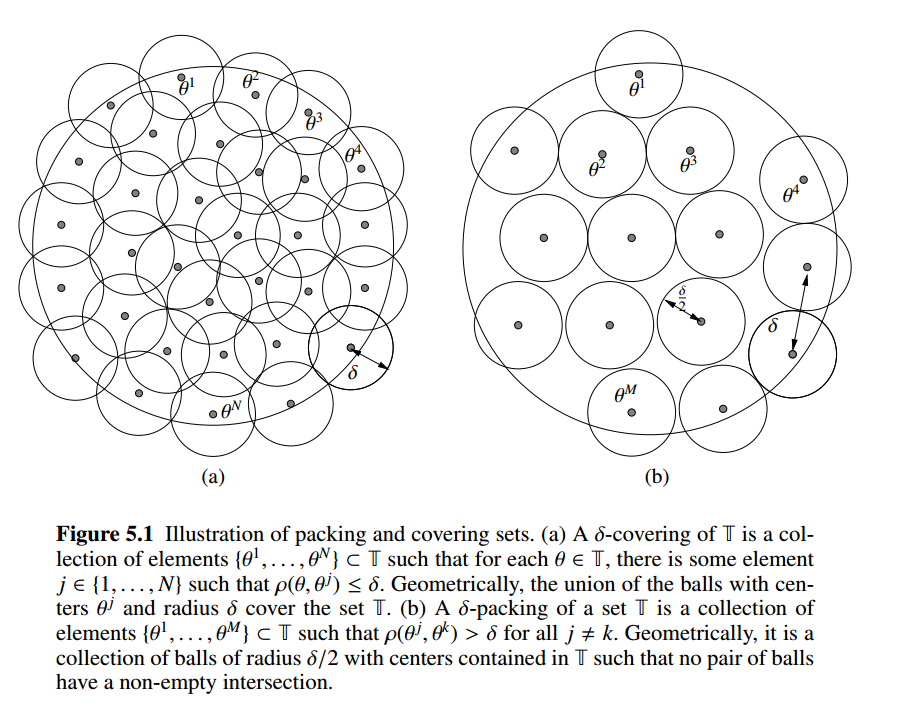
\includegraphics[scale = 0.4]{epsilon_net_covering_packing_number.png}}
\end{minipage}
\caption{\footnotesize{\textbf{The $\epsilon$-net and its associated covering number (a) and packing number (b).  \citep{wainwright2019high}}}}
\label{fig: epsilon_net_covering_packing_number}
\end{figure}

\item \begin{definition} (\textbf{\emph{Covering Numbers}}). \citep{vershynin2018high} \\
\emph{The \textbf{smallest possible cardinality}} of an \emph{$\epsilon$-net} of $K$ is called  \underline{\textbf{\emph{the covering number of $K$}}} and is denoted $\cN(K, d, \epsilon)$. Equivalently, $\cN(K, d, \epsilon)$ is \emph{\textbf{the smallest number} of \textbf{closed balls}} with centers in $K$ and radii $\epsilon$ whose \textbf{\emph{union}} \emph{covers} $K$.
\end{definition}

\item \begin{remark}(\emph{\textbf{Compactness / Precompactness}})\\
An important result in real analysis states that a subset $K$ of a \emph{\textbf{complete metric space}} $(T, d)$ is \underline{\emph{\textbf{precompact}}} (i.e. \emph{the closure of $K$ is compact}) if and only if
\begin{align*}
\cN(K, d, \epsilon) < \infty, \quad \text{ for every }\epsilon > 0.
\end{align*}
Thus we can think about the magnitude $\cN(K, d, \epsilon)$ as \emph{a  \textbf{quantitative measure of compactness} of $K$}.
\end{remark}

\item \begin{definition} (\emph{\textbf{Packing Numbers}}). \citep{vershynin2018high} \\
A subset $\cN$ of a metric space $(T, d)$ is \underline{\emph{\textbf{$\epsilon$-separated}}} if 
\begin{align*}
d(x, y) > \epsilon, \quad \text{ for all distinct }x, y \in \cN.
\end{align*}
\emph{The \textbf{largest possible cardinality}} of an \emph{$\epsilon$-separated} subset of a given set $K \subset T$ is called  \underline{\emph{\textbf{the packing
number of $K$}}} and is denoted $\cP(K, d,  \epsilon)$.
\end{definition}

\item \begin{remark}(\textbf{\emph{Property of Covering Number}})\\
It is easy to see that \emph{the covering number} is \emph{\textbf{non-increasing}} in $\epsilon$, meaning that 
\begin{align*}
\cN(K, d, \epsilon) \ge \cN(K, d, \epsilon'), \quad \text{ whenever } \epsilon \le \epsilon'.
\end{align*} Typically, the covering number \emph{diverges} as $\epsilon \to 0_{+}$, and of interest to us is the
\emph{\textbf{growth rate} of covering number on a \textbf{logarithmic scale}}.
\end{remark}

\item \begin{lemma} \label{lem: covering_maximal}\citep{vershynin2018high}\\
Let $\cN$ be a \textbf{maximal} \textbf{$\epsilon$-separated} subset of $K$, that is, adding more points in $\cN$ will violate the $\epsilon$-separation property. Then $\cN$ is an \textbf{$\epsilon$-net} of $K$.
\end{lemma}
\begin{proof} 
Let $x \in K$; we want to show that there exists $x_0 \in \cN$ such that $d(x, x_0) \le \epsilon$.

If $x \in \cN$, the conclusion is trivial by choosing $x_0 = x$. Suppose now $x \not\in \cN$. The maximality assumption implies that  $\cN \cup \set{x}$ is not $\epsilon$-separated. But this means precisely that 
\begin{align*}
d(x, x_0) \le \epsilon \text{ for some }x_0 \in \cN. \qed
\end{align*}
\end{proof}

\item \begin{remark} (\textbf{\emph{Constructing a Net}}). \citep{vershynin2018high}\\
Lemma above leads to the following  \emph{algorithm} for \emph{constructing an $\epsilon$-net of a given set $K$}:

Choose a point $x_1 \in K$ arbitrarily, choose a point $x_2 \in K$ which is \emph{\textbf{further than $\epsilon$ from $x_1$}}, choose $x_3$ so
that it is \emph{\textbf{further} than $\epsilon$ from \textbf{both} $x_1$ and $x_2$}, and so on. If $K$ is \emph{\textbf{compact}}, the algorithm terminates in \emph{finite time} and gives an $\epsilon$-net of $K$.
\end{remark}

\item \begin{lemma} (\textbf{Equivalence of Covering and Packing Numbers}). \citep{vershynin2018high, wainwright2019high}\\
For any set $K \subset T$ and any  $\epsilon > 0$, we have
\begin{align}
\cP(K, d,  2\epsilon) \le \cN(K, d, \epsilon) \le \cP(K, d,  \epsilon)\label{ineqn: covering_number_packing_number}
\end{align}
\end{lemma}
\begin{proof} The upper bound follows from Lemma \ref{lem: covering_maximal}. For any packing $\cP$ with cardinality $\abs{\cP} = \cP(K, d,  \epsilon)$, $\cP$ is a maximal $\epsilon$-separated set. From Lemma \ref{lem: covering_maximal}, $\cP$ is a \emph{$\epsilon$-net} as well. Then by definition of covering number, $\abs{\cP} \ge \cN(K, d, \epsilon)$.

To prove the lower bound, choose an $2\epsilon$-separated subset $\cP = \set{x_i}_i$ in $K$ and an $\epsilon$-net $\cN = \set{y_j}_j$ of $K$. By the definition of a net, each point $x_i$ belongs \emph{a closed $\epsilon$-ball centered at some point $y_j$}. Moreover, since any closed $\epsilon$-ball can not contain a pair of $2\epsilon$-separated points, \emph{each $\epsilon$-ball centered at $y_j$ may contain \textbf{at most one point} $x_i$}. The \emph{\textbf{pigeonhole principle}} then yields 
\begin{align*}
\abs{\cP} \le \abs{\cN}.
\end{align*}  Since this happens for arbitrary packing $\cP$ and covering $\cN$, the lower bound in the lemma is proved. \qed
\end{proof}

\item \begin{definition} (\textbf{\emph{Metric Entropy}}) \\
\emph{The \textbf{logarithm} of \textbf{the covering numbers}} 
\begin{align*}
\log \cN(K, d, \epsilon)
\end{align*}  is often called \underline{\emph{\textbf{the metric entropy}}} of $K$.
\end{definition}

\item \begin{remark}
When discussing metric entropy, we restrict our attention to subset $K$ of metric spaces $K \subset (T, d)$ that are \emph{\textbf{totally bounded}}, meaning that the covering number $\cN(K, d, \epsilon)$ is \emph{\textbf{finite}} for all $\epsilon > 0$. 

Note that  a \emph{metric space} that is \emph{compact} if and only if it is  \emph{totally bounded} and \emph{complete}. So we can instead assume that $K$ of interest is \emph{compact}.
\end{remark}
\end{itemize}
\subsection{Covering Numbers and Volume}

\subsection{Metric Entropy and Complexity}

\section{Expected Value of Suprema of Empirical Process}
\subsection{Metric Entropy and Sub-Gaussian Processes}
\subsection{Chaining and Dudley's Entropy Integral}
\begin{itemize}
\item \begin{theorem} (\textbf{Dudley's Entropy Integral Inequality}) \citep{vershynin2018high, wainwright2019high}\\
Let $\set{X_{t}, t \in T}$ be a \textbf{zero-mean sub-Gaussian process} with respect to the induced pseudo-metric $d_X$. Then for any $\epsilon \in [0, D]$, where $D  = \sup_{t, t'\in T}d_{X}(t, t')$ we have
\begin{align}
\E{}{\sup_{t, t' \in T}\set{X_t - X_{t'}}} &\le 2\E{}{\sup_{s, s' \in T: d_X(s, s') \le \epsilon}\set{X_s - X_{s'}}} + 32 \int_{\epsilon/4}^{D}\sqrt{\log \cN(T, d_{X}, u)} du \label{ineqn: dudley_metric_entropy_integral_inequality}
\end{align}
\end{theorem}

\item \begin{remark} (\textbf{\emph{Dudley's Entropy Integral Inequality for Symmetrized Empirical Process}}) \\
Define \emph{the zero-mean random variable} 
\begin{align*}
Z_f &:= \frac{1}{\sqrt{n}}\sum_{i=1}^n \epsilon_i f(x_i),
\end{align*} where $\epsilon_i$ are i.i.d. Rademacher random variables and consider the \emph{stochastic process} $\set{Z_f}_{ f \in \cF}$ for $b$-uniformly bounded function class $\cF$, i.e. $\norm{f}{\infty} \le b$ for all $f \in \cF$.

It is straightforward to verify that \emph{the increment} $Z_f - Z_g$ is \emph{\textbf{sub-Gaussian}} with parameter
\begin{align*}
\norm{f - g}{\cP_n}^2 := \frac{1}{n}\sum_{i=1}^n\paren{f(x_i) - g(x_i)}^2.
\end{align*}
Consequently, by \emph{Dudley's entropy integral}, we have
\begin{align}
\E{\epsilon}{\sup_{f\in \cF}\abs{\frac{1}{n}\sum_{i=1}^n \epsilon_i f(x_i) }} &\le \frac{24}{\sqrt{n}}\int_{0}^{2b}\sqrt{\log \cN(\cF, \norm{\cdot}{\cP_n}, t)} dt, \label{ineqn: dudley_metric_entropy_Rademacher_process}
\end{align}
where we have used the fact that $\sup_{f, g \in \cF}\norm{f - g}{\cP_n} \le 2b$. Finally, by \emph{symmetrization}, 
\begin{align*}
\E{X}{\sup_{f \in \cF}\abs{\frac{1}{n}\sum_{i=1}^{n}f(X_i) - \E{}{f(X)}}} &\le 2 \E{X}{\E{\epsilon}{\sup_{f\in \cF}\abs{\frac{1}{n}\sum_{i=1}^n \epsilon_i f(X_i) }| X_1 \xdotx{,} X_n}}\\
&\le \frac{48}{\sqrt{n}}\int_{0}^{2b}\sqrt{\log \cN(\cF, \norm{\cdot}{\cP_n}, t)} dt.
\end{align*}
\end{remark}
\end{itemize}
\subsection{Vapnik-Chervonenkis Class}
\begin{itemize}
\item \begin{theorem} (\textbf{Covering Numbers via VC Dimension}).  \citep{vershynin2018high}\\
Let $\cF$ be a class of \textbf{binary} functions  on a probability space $(\cX, \srF, \cP)$. Then, for every $\epsilon \in (0, 1)$, we
have
\begin{align}
\cN(\cF, L_2(\cP), \epsilon) &\le \paren{\frac{2}{\epsilon}}^{Cd}, \label{ineqn: covering_number_bound_vc_dimension}
\end{align} where $d = \text{VC-Dim}(\cF)$.
\end{theorem}

\item  \begin{theorem} (\textbf{Empirical Processes via VC dimension}).  \citep{vershynin2018high}\\
Let $\cF$ be a class of \textbf{binary} functions  on a probability space $(\cX, \srF, \cP)$ with \textbf{finite VC dimension} $d \ge 1$. Let $X, X_1 \xdotx{,} X_n$ be \textbf{independent} random variables in $\cX$ distributed according to the law $\cP$. Then 
\begin{align}
\E{}{\sup_{f \in \cF}\abs{\frac{1}{n}\sum_{i=1}^{n}f(X_i) - \E{}{f(X)}}} &\le C\sqrt{\frac{d}{n}}, \label{ineqn: expected_emp_process_vc_dimension}
\end{align} where $d = \text{VC-Dim}(\cF)$.
\end{theorem}


\item \begin{remark} (\textbf{\emph{The Classical Glivenko-Cantelli Theorem, Non-Asymptotic Version}})\\
Consider the \emph{classical Glivenko-Cantelli theorem} \eqref{eqn: gilvenko_cantelli}, which amounts to bounding
\begin{align*}
\norm{\widehat{F}_n - F}{\infty} :=  \sup_{t\in \bR}\abs{\widehat{F}_n(t) - F(t)}.
\end{align*}
Since \emph{the set of indicator functions has VC dimension} $d = 1$, apply inequality \eqref{ineqn: expected_emp_process_vc_dimension} above, we have
\begin{align}
\E{}{ \sup_{t\in \bR}\abs{\widehat{F}_n(t) - F(t)}} &\le C\sqrt{\frac{1}{n}} \label{ineqn: gilvenko_cantelli_expected_value}
\end{align} Thus combing with  \emph{the functional Hoeffding inequality} \eqref{ineqn: hoeffding_inequality_functional}, we conclude that for any $\delta >0$, with probabilty at least $1-\delta$, 
\begin{align}
 \sup_{t\in \bR}\abs{\widehat{F}_n(t) - F(t)} &\le  \frac{c + \sqrt{8 \log(2/\delta)}}{\sqrt{n}}  \label{ineqn: gilvenko_cantelli}
\end{align} where $c$ is a universal constant. Apart from better constants, this bound is \emph{unimprovable}.
\end{remark}
\end{itemize}
\subsection{Comparison Theorems}




\newpage
\bibliographystyle{plainnat}
\bibliography{reference.bib}
\end{document}